\documentclass{beamer}

% Theme
\usetheme{Madrid}
\usecolortheme{default}
\setbeamertemplate{navigation symbols}{}
\setbeamertemplate{bibliography entry title}{}
% Packages
\usepackage{amsmath, amssymb}
\usepackage{graphicx}
\nocite{*}
\bibliographystyle{plain}  % or another style like alpha, ieeetr, etc.
% Title Page
\title[Implicit Loss Fine-Tuning]{Fine-tuning with implicit loss}
\author{Lukasz Adamowicz}
% \institute[Heidelberg University]{M2 Mathématiques, Modélisation et Apprentissage \\ Internship at Hamprecht Lab, IWR Heidelberg}
\date{August 28, 2025}

\begin{document}

% Title slide
\begin{frame}
  \titlepage
\end{frame}

% Outline
\begin{frame}{Outline}
  \tableofcontents
\end{frame}


%------------------------------------------------------
\section{Problem Statement}
\begin{frame}{General Optimization Problem}
  \begin{itemize}
    \item Energy model: $E(\theta, M, p)$.
    \item Ground state density coefficients $p_{\theta}$ are fixed points:
    \[
      p_{\theta,i} = \arg\min_{p:\langle w,p \rangle = N} E(\theta, M, p).
    \]
    \item Loss: $L(\theta) = \sum_{i=1}^{n} L_i(p_{\theta,i}) = \sum_{i=1}^{n} \frac{1}{2} \|p_{\theta,i} - p_{gs,i}\|^2$.
    \item Bilevel optimization problem across multiple molecules.
    \item Challenge: compute gradient of $L(\theta)$ with respect to model parameters.
  \end{itemize}
\end{frame}

\begin{frame}{Single Molecule Optimization Problem}
  \begin{itemize}
    \item For a single molecule $M$:
    \item Fixed point equation: $p_{\theta} = \arg\min_{p:\langle w,p \rangle = N} E(\theta, p)$.
    \item Loss: $L(\theta) = L(p_{\theta}) = \frac{1}{2}\|p_{\theta} - p_{gs}\|^2$.
    \item Goal: Find $\theta^* = \arg\min_{\theta} L(\theta)$.
    \item Need to compute $\frac{dL}{d\theta}$ without direct differentiation through the fixed point finding process.
  \end{itemize}
\end{frame}

%------------------------------------------------------
\section{Jacobian Approach}
\begin{frame}{Jacobian Approach}
  \begin{itemize}
    \item Based on implicit function theorem.
    \item Gradient formula:
    \[
      \frac{\partial L(p_{\theta})}{\partial \theta} = -(p_{\theta}-p_{gs}) \cdot \left(\frac{\partial}{\partial p}\mathcal{P}\nabla_p E(\theta, p)\right)^{-1} \cdot \frac{\partial}{\partial \theta}\big(\mathcal{P}\nabla_p E(\theta, p)\big)
    \]
    \item  $\mathcal{P}$ is the projection operator onto subspace $\langle w,p \rangle = N$.
    \item we solve for $y = -(p_{\theta}-p_{gs}) \cdot \left(\frac{\partial}{\partial p}\mathcal{P}\nabla_p E(\theta, p)\right)^{-1}$
    \item Memory and stability issues.
  \end{itemize}
\end{frame}

\begin{frame}{Jacobian Results}
  \begin{itemize}
    \item Training loss sometimes decreases, but diverges later.
    \item Conjugate gradient method failed.
    \item Did not improve density difference.
    \item Jacobian has big spread of eigenvalues values
  \end{itemize}
\end{frame}

\begin{frame}
 \begin{center}
    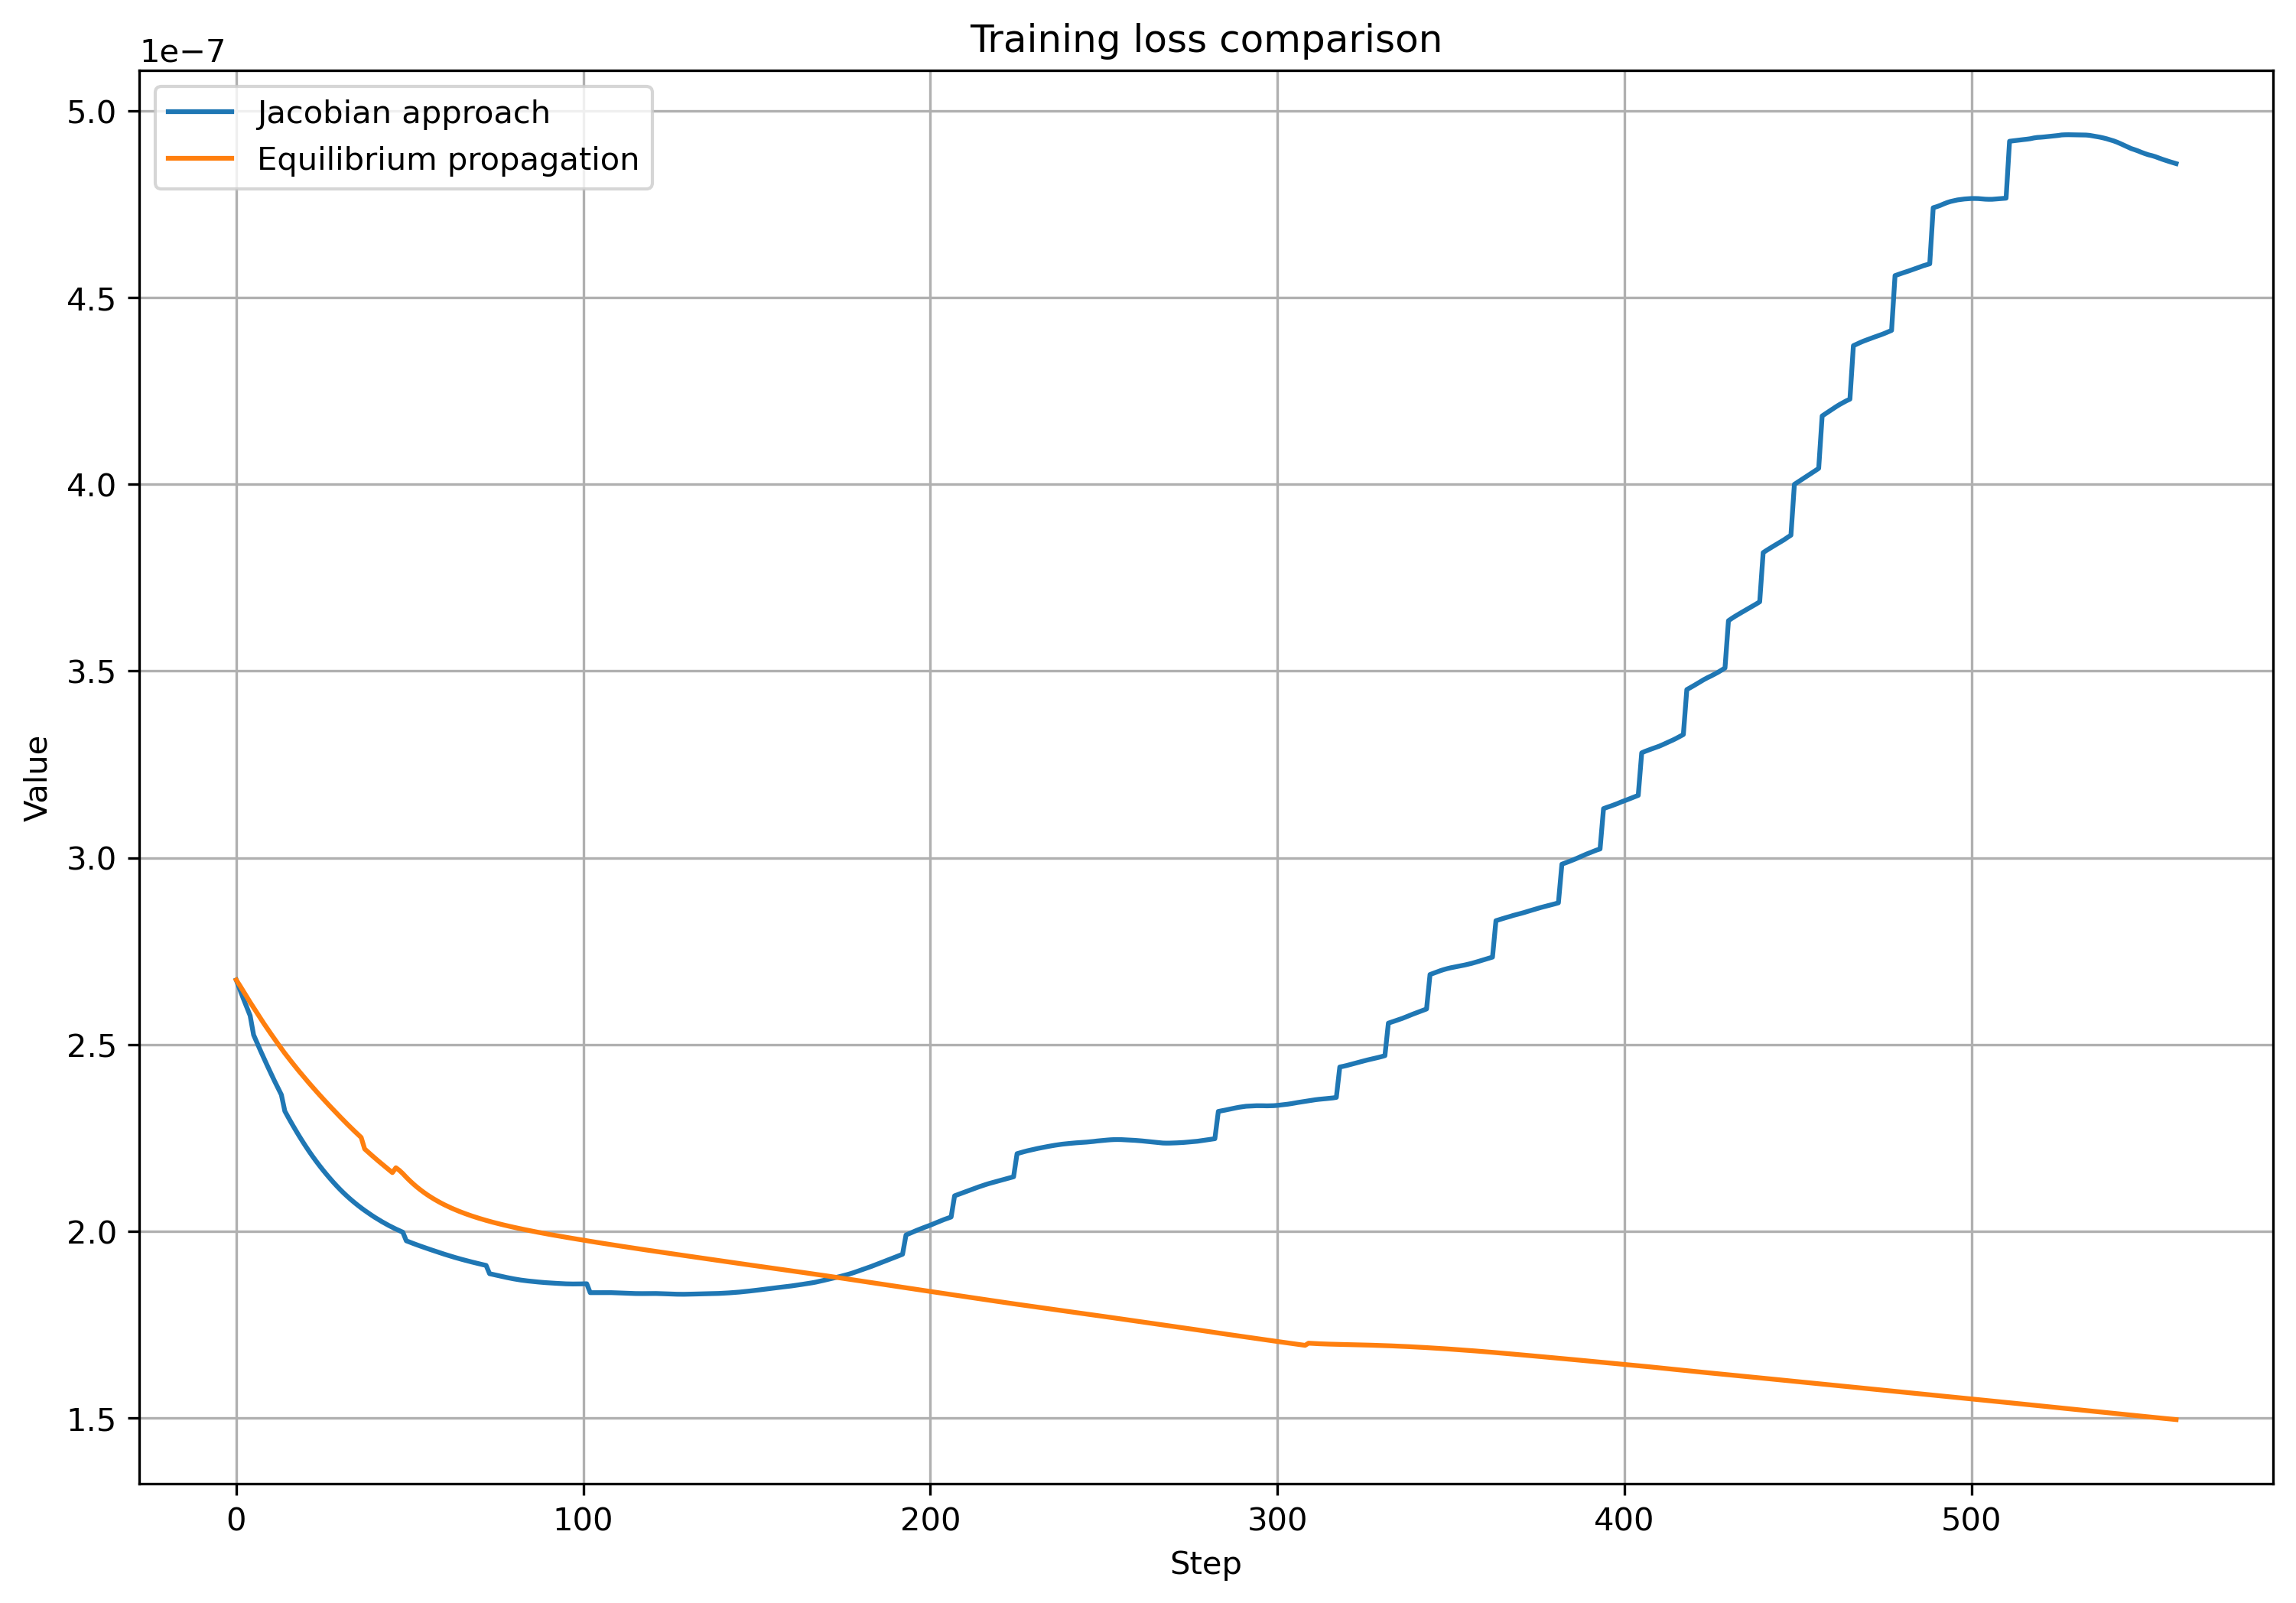
\includegraphics[width=0.8\textwidth]{images/loss_comparison.png} % Jacobian vs EqProp training loss
  \end{center}
\end{frame}


%------------------------------------------------------
\section{Equilibrium Propagation}
\begin{frame}{Equilibrium Propagation}
  \begin{itemize}
    \item Alternative gradient estimation method.
    \item Define total energy: $T(\theta, p, \beta) = E(\theta, p) + \beta L(p)$.
    \item Define $p_{\theta}^{\beta}$ as the fixed point:
    \[
      p_{\theta}^{\beta} = \arg\min_{p:\langle w,p \rangle = N} T(\theta, p, \beta) = \arg\min_{p:\langle w,p \rangle = N} [E(\theta, p) + \beta L(p)]
    \]
    \item Gradient formula:
    \[
      \frac{d}{d\theta} L(p_{\theta}) = \lim_{\beta \to 0} \frac{1}{\beta} \Big[ \partial_{\theta}T(\theta, p^{\beta}_{\theta}, \beta) - \partial_{\theta}T(\theta, p^{0}_{\theta}, 0) \Big].
    \]
  \end{itemize}
\end{frame}

\begin{frame}{Equilibrium Propagation Results}
  \begin{itemize}
    \item Worked for fine-tuning on single molecule.
    \item Loss decreased consistently.
    \item Density difference decreased, but energy difference increases
  \end{itemize}

\end{frame}

\begin{frame}
   \begin{center}
    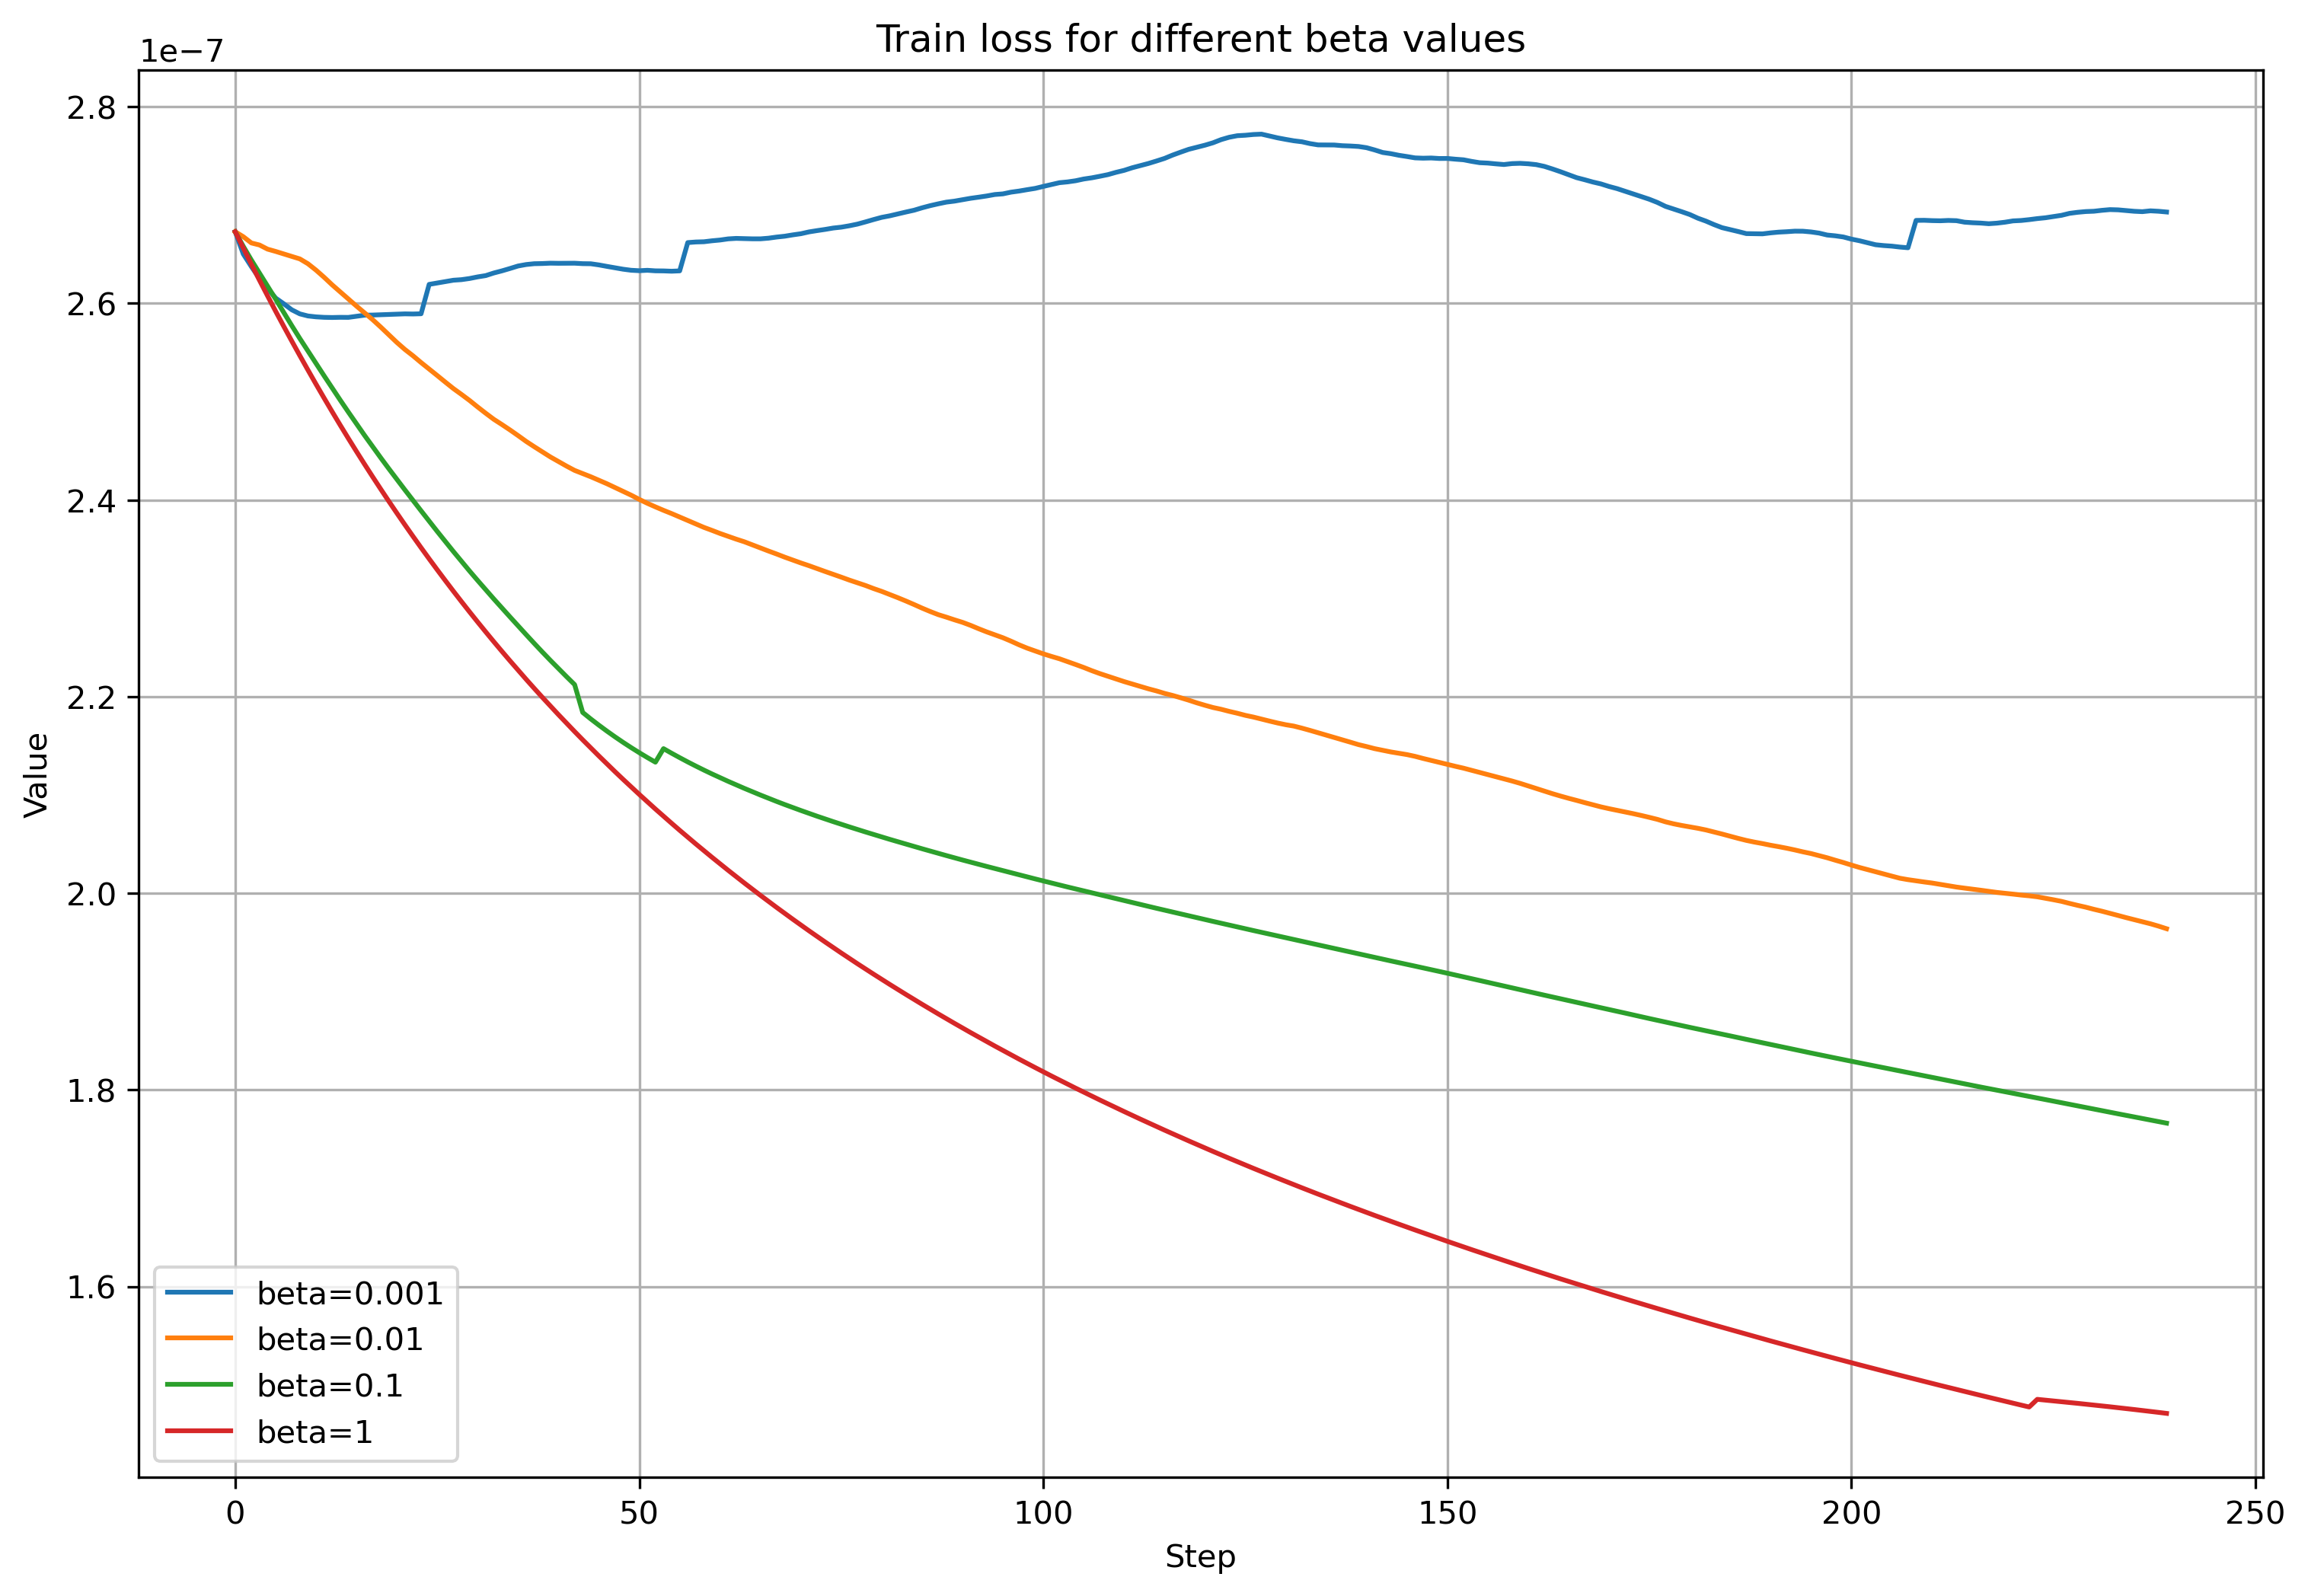
\includegraphics[width=0.8\textwidth]{images/train_loss_betas.png} % EqProp with different beta
  \end{center}
\end{frame}

%------------------------------------------------------
\section{Stability Issues and Fixed Point Correction}
\begin{frame}{Stability Issues}
  \begin{itemize}
    \item Training stability deteriorates over time (known issue in DEQ models).
    \item Fixed point search takes longer and longer during training.
    \item There are techniques for alleviating the issue
  \end{itemize}
\end{frame}

\begin{frame}{Fixed Point Correction (Original Contribution)}
  \begin{itemize}
    \item Technique: include intermediate trajectory points in loss.
    \item Loss function:
    \[
      L_{FPC}(\theta) = \sum_{k} \gamma^{n-k} L(p_{i_k}),
    \]
    where $p_{i_k}$ are intermediate points.
    \item Helps stabilize training, but may reduce performance.
    \item I modified it to be random
  \end{itemize}

\end{frame}

\begin{frame}
   \begin{center}
    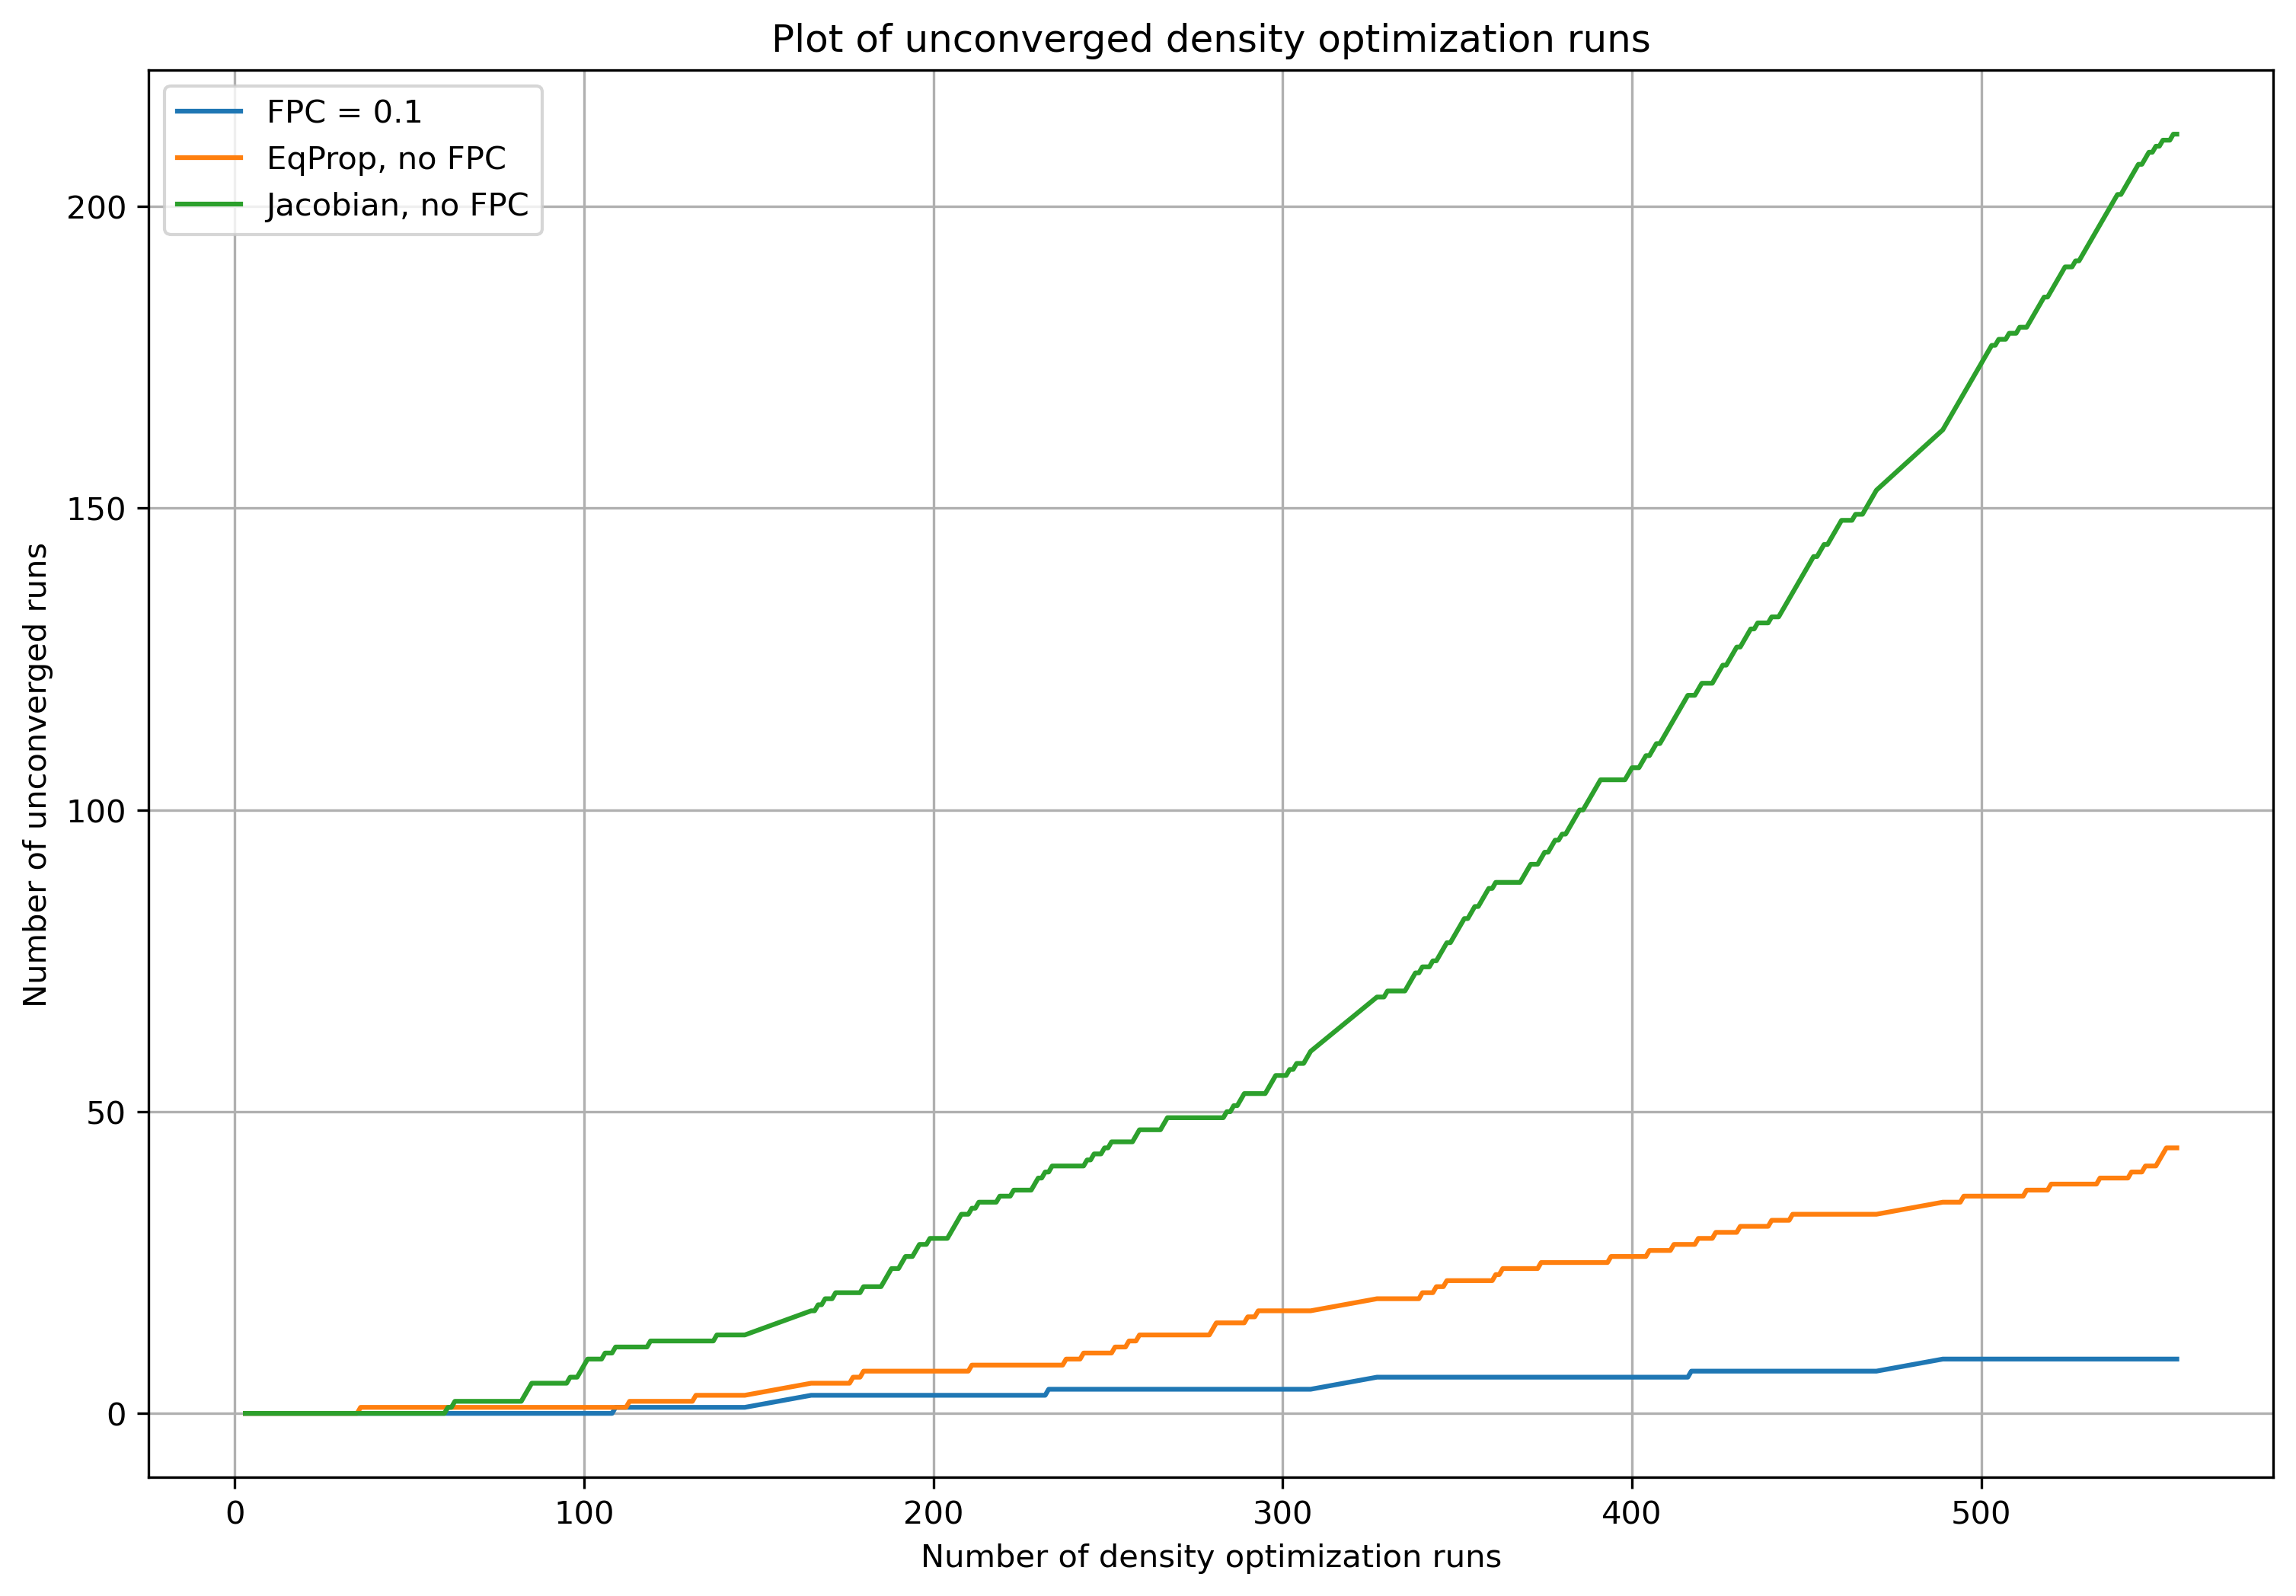
\includegraphics[width=0.8\textwidth]{images/stability_plot.png} % Stability plot
  \end{center}
\end{frame}

%------------------------------------------------------
\section{Conclusions}
\begin{frame}{Conclusions}
  \begin{itemize}
    \item Jacobian approach: not effective for now, would be nice if it works
    \item Equilibrium propagation: potentially viable
    \item Training is very unstable and very slow

  \end{itemize}
\end{frame}

\begin{frame}{End}
\begin{center}
 Thanks for coming
\end{center}
\end{frame}
\begin{frame}[allowframebreaks]{References}
\nocite{*}
\bibliographystyle{plain}
\bibliography{./references.bib}
\end{frame}

%------------------------------------------------------
\appendix
\section{Appendix}
\begin{frame}{Jacobian Gradient Derivation - Part 1}
  \begin{itemize}
    \item Starting from loss function: $L(\theta) = \frac{1}{2}\|p_{\theta} - p_{gs}\|^2$.
    \item Using chain rule: $\frac{\partial L}{\partial \theta} = \frac{\partial L}{\partial p_{\theta}} \cdot \frac{\partial p_{\theta}}{\partial \theta}$.
    \item First term is straightforward: $\frac{\partial L}{\partial p_{\theta}} = (p_{\theta} - p_{gs})$.
    \item For second term, we need the implicit function theorem.
  \end{itemize}
\end{frame}

\begin{frame}{Jacobian Gradient Derivation - Part 2}
  \begin{itemize}
    \item At fixed point, we have: $\mathcal{P}\nabla_p E(\theta, p_{\theta}) = 0$.
    \item Differentiating this constraint with respect to $\theta$:
    \begin{align}
      \frac{\partial}{\partial \theta}\left[\mathcal{P}_{\langle w,p \rangle = N}\nabla_p E(\theta, p_{\theta})\right] &= 0 \\
      \frac{\partial}{\partial p}\mathcal{P}_{\langle w,p \rangle = N}\nabla_p E(\theta, p_{\theta}) \cdot \frac{\partial p_{\theta}}{\partial \theta} + \frac{\partial}{\partial \theta}\mathcal{P}_{\langle w,p \rangle = N}\nabla_p E(\theta, p_{\theta}) &= 0
    \end{align}
    \item Solving for $\frac{\partial p_{\theta}}{\partial \theta}$:
    \begin{align}
      \frac{\partial p_{\theta}}{\partial \theta} &= -\left(\frac{\partial}{\partial p}\mathcal{P}_{\langle w,p \rangle = N}\nabla_p E(\theta, p_{\theta})\right)^{-1} \cdot \frac{\partial}{\partial \theta}\mathcal{P}_{\langle w,p \rangle = N}\nabla_p E(\theta, p_{\theta})
    \end{align}
  \end{itemize}
\end{frame}

\begin{frame}{Jacobian Gradient Derivation - Part 3}
  \begin{itemize}
    \item Substituting back into our chain rule formula:
    \begin{align}
      \frac{\partial L}{\partial \theta} &= (p_{\theta} - p_{gs})^T \cdot \frac{\partial p_{\theta}}{\partial \theta} \\
      &= -(p_{\theta} - p_{gs}) \cdot \left(\frac{\partial}{\partial p}\mathcal{P}_{\langle w,p \rangle = N}\nabla_p E(\theta, p_{\theta})\right)^{-1} \cdot \frac{\partial}{\partial \theta}\mathcal{P}_{\langle w,p \rangle = N}\nabla_p E(\theta, p_{\theta})
    \end{align}
    \item The term $\frac{\partial}{\partial p}\mathcal{P}_{\langle w,p \rangle = N}\nabla_p E(\theta, p_{\theta})$ is the projected Hessian matrix of the energy function.
  \end{itemize}
\end{frame}

\begin{frame}{Equilibrium Propagation Derivation - Part 1}
  \begin{itemize}
    \item Define perturbed energy function: $T(\theta,p,\beta)=E(\theta,p)+\beta L(p)$.
    \item Define $p_{\theta}^{\beta}$ as the fixed point of this perturbed energy:
    \[
      p_{\theta}^{\beta} = \arg\min_{p:\langle w,p \rangle = N} T(\theta, p, \beta)
    \]
    \item Note that $p_{\theta}^{0} = p_{\theta}$ (the original fixed point).
    \item Our goal: compute $\frac{d}{d\theta}L(p_{\theta})$.
  \end{itemize}
\end{frame}

\begin{frame}{Equilibrium Propagation Derivation - Part 2}
  \begin{itemize}
    \item Define function $G(\theta,\beta) = L(p_{\theta}^{\beta})$.
    \item There's symmetry of second derivatives $\frac{d}{d\beta}\frac{d}{d\theta} $ at $\beta = 0, \theta = \theta$

  \end{itemize}
\end{frame}

\begin{frame}{Equilibrium Propagation Derivation - Part 3}
  \begin{itemize}
    \item $\frac{dG}{d\beta×} = \frac{\partial T}{\partial \beta} + \frac{\partial T}{\partial p} \frac{d p_\theta^\beta}{d\beta×},$ but the second term vanishes at $p = p_\theta^\beta$.
    \item $ \frac{\partial T}{\partial \beta}\big|_{\beta = 0} = L(p_\theta)$
  \end{itemize}
\end{frame}



\end{document}
